\documentclass[12pt,utf8]{beamer}

% Gute Einführung zu LaTeX-Beamer: http://www2.informatik.hu-berlin.de/~mischulz/beamer.html

%-----PARAMETERS-----

%Wichtige Standard Pakete!
%\usepackage[german]{babel}
\usepackage{ngerman}
\usepackage{xcolor}
\usepackage{graphicx}
%\usepackage{subcaption}
\usepackage{tikz}


%Für den Header notwendig!
%\usepackage[percent]{overpic}

\usepackage{hyperref} % für korrekte Links

%Einbinden des Themes
\input{design_latex-template/beamerthemeFOSSAG.sty}


%Standard Angaben
\title{
	\hspace*{8cm}
	
\includegraphics[scale=0.2]{resources/logo_500px.png}
	\newline
	FOSS-AG
}
\subtitle{Git}
\author{@chef\_excellence}
\institute[FOSS AG]{\textbf{F}ree and \textbf{O}pen \textbf{S}ource \textbf{S}oftware \textbf{AG}}


\date{\today}

%-----IMPLEMENTATION-----
\begin{document}
	\begin{frame}
		\titlepage
	\end{frame}

	\begin{frame}
		\begin{figure}
			\centering
			
\includegraphics[scale=0.1]{resources/cc.png}
			
\includegraphics[scale=0.1]{resources/by.png}
			
\includegraphics[scale=0.1]{resources/sa.png}
		\end{figure}
		\centering
		Attribution-ShareAlike 4.0 International\\(CC BY-SA 4.0) 
	\end{frame}

	\begin{frame}
		\frametitle{Was ist Git?}
		\begin{itemize}
			\item Version Control System
			\item erlaubt verteilte Softwareentwicklung
		\end{itemize}
	\end{frame}

	\begin{frame}
		\begin{figure}
			\centering
			
\includegraphics[scale=0.5]{resources/subversion.png}
			
\includegraphics[scale=0.2]{resources/git.png}
			
			
\includegraphics[scale=0.6]{resources/mercurial.png}
			
			\tiny{\cite{subversion}}
			\tiny{\cite{git_logo}}
			\tiny{\cite{mercurial}}
		\end{figure}
	\end{frame}

	\begin{frame}
		\frametitle{Was macht Git anders?}
		\centering
		In a nutshell:\\
		\textbf{Snapshots statt Diffs}
	\end{frame}

	\begin{frame}
		\frametitle{Diffs}
		\begin{figure}[h]
			\centering
			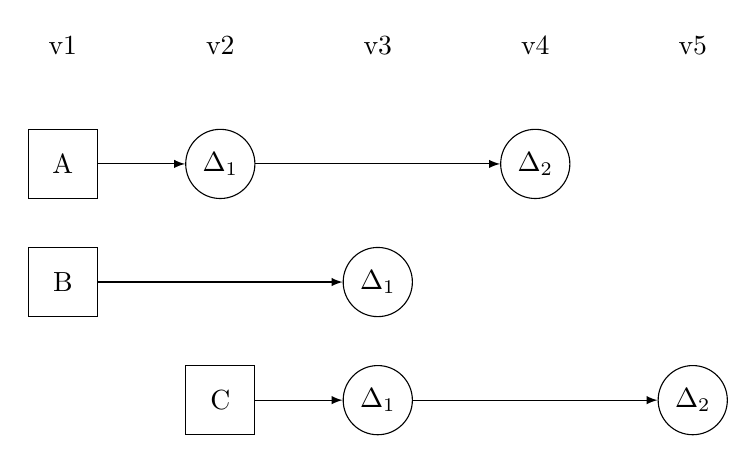
\begin{tikzpicture}
				\tikzstyle{version} = []
				\tikzstyle{file}=[draw, minimum size=25pt]
				\tikzstyle{diff}=[circle, draw, minimum size=25pt]
				\tikzset{edge/.style = {->,> = latex}}
				
				% versions
				\node[version](v1) at (0,1.5) {v1};
				\node[version](v2) at (2,1.5) {v2};
				\node[version](v3) at (4,1.5) {v3};
				\node[version](v4) at (6,1.5) {v4};
				\node[version](v5) at (8,1.5) {v5};
				
				% file A + diffs			
				\node[file](A)   at (0,0) {A};
				\node[diff](DA1) at (2,0) {$\Delta_1$};
				\node[diff](DA2) at (6,0) {$\Delta_2$};
				\draw[edge](A)   to (DA1);
				\draw[edge](DA1) to (DA2);
				
				% file B + diffs
				\node[file](B)   at (0,-1.5) {B};
				\node[diff](DB1) at (4,-1.5) {$\Delta_1$};
				\draw[edge](B)   to (DB1);
				
				% file C + diffs
				\node[file](C)   at (2,-3) {C};
				\node[diff](DC1) at (4,-3) {$\Delta_1$};
				\node[diff](DC2) at (8,-3) {$\Delta_2$};
				\draw[edge](C)   to (DC1);
				\draw[edge](DC1) to (DC2);
			\end{tikzpicture}
		\end{figure}
	\end{frame}
	
	\begin{frame}
		\frametitle{Snapshots}
		\begin{figure}[h]
			\centering
			\begin{tikzpicture}
			\tikzstyle{version} = []
			\tikzstyle{file}=[draw, minimum size=25pt]
			\tikzstyle{link} = [dash pattern=on 3pt off 3pt, draw, minimum size=25pt]
			\tikzset{edge/.style = {-,> = latex, dashed}}
			
			% versions
			\node[version](v1) at (0,1.5) {v1};
			\node[version](v2) at (2,1.5) {v2};
			\node[version](v3) at (4,1.5) {v3};
			\node[version](v4) at (6,1.5) {v4};
			\node[version](v5) at (8,1.5) {v5};
			
			% file A + diffs
			\node[file](A)   	at (0,0) {A};
			\node[file](A1)  	at (2,0) {A$_1$};
			\node[link](linkA1) at (4,0) {A$_1$};
			\node[file](A2)  	at (6,0) {A$_2$};
			\node[link](linkA2)	at (8,0) {A$_2$};
			\draw[edge](linkA1) to (A1);
			\draw[edge](linkA2) to (A2);
			
			% file B + diffs
			\node[file](B)   	 at (0,-1.5) {B};
			\node[link](linkB)	 at (2,-1.5) {B};
			\node[file](B1) 	 at (4,-1.5) {B$_1$};
			\node[link](linkB1)  at (6,-1.5) {B$_1$};
			\node[link](link1B1) at (8,-1.5) {B$_1$};
			\draw[edge](linkB) 	 to (B);
			\draw[edge](linkB1)  to (B1);
			\draw[edge](link1B1) to (linkB1);
			
			% file C + diffs
			\node[file](C)   	at (2,-3) {C};
			\node[file](C1)  	at (4,-3) {C$_1$};
			\node[link](linkC1)	at (6,-3) {C$_1$};
 			\node[file](C2) 	at (8,-3) {C$_2$};
			\draw[edge](linkC1)	to (C1);
			\end{tikzpicture}
		\end{figure}
	\end{frame}

	% Vorteile von Snapshots sind besonders stark, wenn es um Branching geht

	\begin{frame}
		\frametitle{Git ist schnell!}
		\begin{itemize}
			\item Geschwindigkeitsvorteil gegenueber vielen anderen VCSs
			\item Fast alle Operationen finden lokal statt und benoetigen keine Kommunikation mit einem Server
			\begin{itemize}
				\item Git-History durchsuchen
				\item auf ein alte Revision wechseln
				\item Aenderungen am Projekt commiten
			\end{itemize}
			\item[$\Rightarrow$] Kein Overhead durch Netzwerkkommunikation
		\end{itemize}
	\end{frame}
	
	\begin{frame}
		\frametitle{Support your local repo}
		\begin{itemize}
			\item Arbeiten und commiten auf lokaler Kopie des Projekts
			\item \texttt{git push} schiebt Aenderung auf den Server
			\item[$\Rightarrow$] erlaubt dezentralisiertes und lokales Arbeiten 
		\end{itemize}
	\end{frame}
	
	\begin{frame}
		\frametitle{Git vs. SVN}
		\begin{itemize}
			\item Aenderungen der Datei sind offline moeglich
			\item keine lokalen Commits moeglich
			\item \texttt{svn commit} = \texttt{git commit + git push}
		\end{itemize}
	\end{frame}

	\begin{frame}
		\frametitle{Die Dreifaltigkeit Gits}
		Jede Datei im Repository hat einen von drei Zustaende:
		\begin{itemize}
			\item Modified\\
				Die Datei wurde veraendert und entspricht nicht mehr der Version des momentanen Snapshots
			\item Staged\\
				Die Datei wurde fuer den naechsten Commit vorgemerkt und wird Teil des naechsten Snapshots
			\item Commited\\
				Die Datei wurde zum neuen Snapshot hinzugefuegt und ist in der lokalen Datenbank gespeichert
		\end{itemize}
	\end{frame}

	\begin{frame}
		\frametitle{Grundlegender Workflow}
		\begin{enumerate}
			\item Hack Hack Hack
			\item Hinzufuegen der veraenderten Dateien zur Staging Area\\
				\texttt{git add FILES}
			\item Erstellen des neuen Snapshots (lokal)\\
				\texttt{git commit -m COMMIT\_MESSAGE}
			\item Schiebe alle Aenderungen auf den Server\\
				\texttt{git push}
		\end{enumerate}
	\end{frame}

	\begin{frame}
	\frametitle{Statusbericht}
		\begin{itemize}
			\item Der Zustand der Dateien kann mit \texttt{git status -s} ueberprueft werden\\
			\item Zeigt zusaetzlich auch Dateien an, die nicht zum Projekt gehoeren (untracked files)
		\end{itemize}
	\end{frame}

	\begin{frame}
		\begin{figure}
			
\includegraphics[scale=0.6]{resources/sponge.jpg}
			
			\tiny{\cite{sponge}}
		\end{figure}
	\end{frame}
	
	\begin{frame}
		\frametitle{.gitignore}
		Manche Dateien will man bewusst nicht hinzufuegen
		\begin{itemize}
			\item[$\Rightarrow$] \texttt{.gitignore}
			\begin{itemize}
				\item Fuege einzelne Dateien hinzu, die von Git ignoriert werden sollen
				\item Regulaere Ausdruecke koennen verwendet werden, um z.B. alle Dateien eines bestimmten Formats auszuschliessen
			\end{itemize}
		\end{itemize}
		Sammlung an Templates: \url{https://github.com/github/gitignore}
	\end{frame}

	\begin{frame}
		\frametitle{Branching}	
		\begin{itemize}
			\item Fast jedes VCS hat eine Art des Branching
			\item Git's Branching ist leichtgewichtig und schnell!
			\item Kein Kopieren von Dateien nötig!
		\end{itemize}
	\end{frame}

	\begin{frame}
		\frametitle{Branching - Beispiel}
		Unser Projekt besteht aus 3 Dateien:
		\begin{itemize}
			\item[] \texttt{README}
			\item[] \texttt{LICENSE}
			\item[] \texttt{test.rb}
		\end{itemize}
	
		\texttt{git add README LICENSE test.rb}\\
		\texttt{git commit -m 'The initial commit of my project'}
	\end{frame}
	
	\begin{frame}
		\begin{figure}
			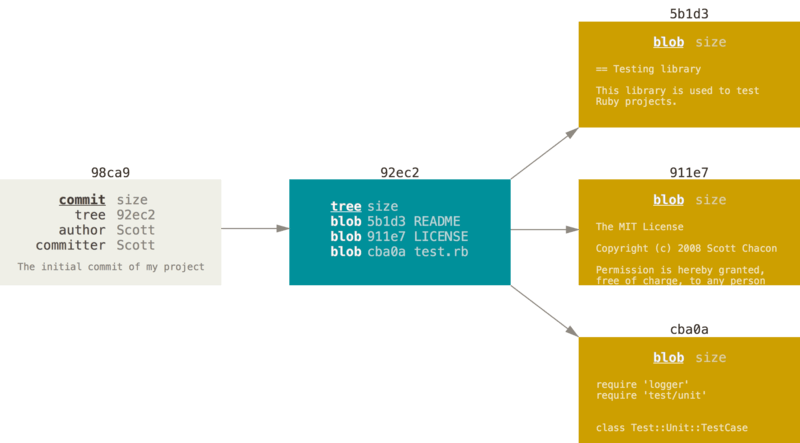
\includegraphics[scale=0.4]{resources/commit-and-tree.png}
			
			\tiny{\cite{commit-and-tree}}
		\end{figure}
	\end{frame}

	\begin{frame}
		\begin{figure}
			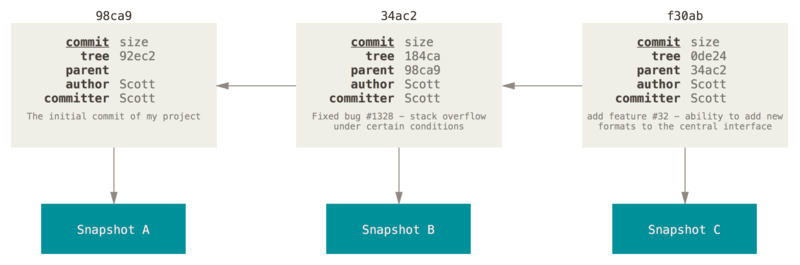
\includegraphics[scale=0.4]{resources/commits-and-parents.png}
			
			\tiny{\cite{commit-and-parents}}
		\end{figure}
	\end{frame}

	\begin{frame}
		\frametitle{Branching - Beispiel}
		\begin{itemize}
			\item Jeder Commit wird als Baum repraesentiert, der Informationen ueber den jeweiligen Snapshot abspeichert
			\begin{itemize}
				\item Autor
				\item Commit message
				\item Hashes
			\end{itemize}
			\item Jeder Commit wird an die Liste der bisherigen Commits angefuegt
		\end{itemize}
		$\Rightarrow$ ein Branch ist ein Pointer auf einen Commit
	\end{frame}

	\begin{frame}
		\frametitle{HEAD-master}
		\begin{itemize}
			\item \texttt{master}:\\
				Keine besondere Stellung!\\
				Bennenung erfolgt automatisch durch \texttt{git init}
			\item \texttt{HEAD}:\\
				Zeiger auf den Branch auf dem man lokal arbeitet.
		\end{itemize}
	\end{frame}

	\begin{frame}
		\begin{figure}[h]
			\centering
			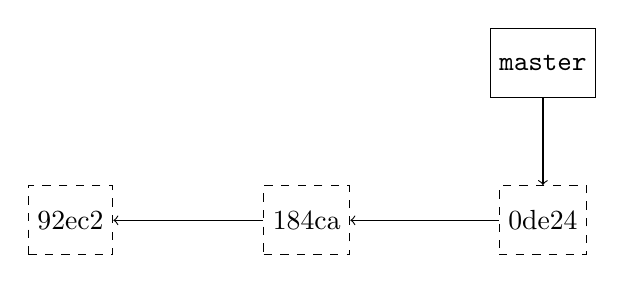
\begin{tikzpicture}
			\tikzstyle{version} = []
			\tikzstyle{branch}=[draw, minimum size=25pt]
			\tikzstyle{commit} = [dash pattern=on 3pt off 3pt, draw, minimum size=25pt]
			\tikzset{edge/.style = {-,-> = latex}}

			\node[commit](commit1) at (0,0) {92ec2};
			\node[commit](commit2) at (3,0) {184ca};
			\node[commit](commit3) at (6,0) {0de24};
			\draw[edge](commit2) to (commit1);
			\draw[edge](commit3) to (commit2);
			
			\node[branch](master) at (6,2) {\texttt{master}};
			\draw[edge](master) to (commit3);

			\end{tikzpicture}
		\end{figure}
	\end{frame}

	\begin{frame}
		\begin{figure}[h]
			\centering
			\begin{tikzpicture}
			\tikzstyle{head} = []
			\tikzstyle{branch}=[draw, minimum size=25pt]
			\tikzstyle{commit} = [dash pattern=on 3pt off 3pt, draw, minimum size=25pt]
			\tikzset{edge/.style = {-,-> = latex}}
			
			\node[commit](commit1) at (0,0) {92ec2};
			\node[commit](commit2) at (3,0) {184ca};
			\node[commit](commit3) at (6,0) {0de24};
			\draw[edge](commit2) to (commit1);
			\draw[edge](commit3) to (commit2);
			
			\node[branch](master) at (6,2) {\texttt{master}};
			\draw[edge](master) to (commit3);
			
			\node[head](head) at (6,4) {\texttt{HEAD}};
			\draw[edge](head) to (master);
			
			\end{tikzpicture}
		\end{figure}
	\end{frame}

	\begin{frame}
		\begin{figure}[h]
			\centering
			\begin{tikzpicture}
			\tikzstyle{head} = []
			\tikzstyle{branch}=[draw, minimum size=25pt]
			\tikzstyle{commit} = [dash pattern=on 3pt off 3pt, draw, minimum size=25pt]
			\tikzset{edge/.style = {-,-> = latex}}
			
			\node[commit](commit1) at (0,0) {92ec2};
			\node[commit](commit2) at (3,0) {184ca};
			\node[commit](commit3) at (6,0) {0de24};
			\draw[edge](commit2) to (commit1);
			\draw[edge](commit3) to (commit2);
			
			\node[branch](master) at (6,2) {\texttt{master}};
			\draw[edge](master) to (commit3);
			
			\node[branch](testing) at (6,-2) {\texttt{testing}};
			\draw[edge](testing) to (commit3);
			
			\node[head](head) at (6,4) {\texttt{HEAD}};
			\draw[edge](head) to (master);
			
			\end{tikzpicture}
		\end{figure}
		Erstellen eines \texttt{testing} Branch.
	\end{frame}

	\begin{frame}
		\begin{figure}[h]
			\centering
			\begin{tikzpicture}
			\tikzstyle{head} = []
			\tikzstyle{branch}=[draw, minimum size=25pt]
			\tikzstyle{commit} = [dash pattern=on 3pt off 3pt, draw, minimum size=25pt]
			\tikzset{edge/.style = {-,-> = latex}}
			
			\node[commit](commit1) at (0,0) {92ec2};
			\node[commit](commit2) at (3,0) {184ca};
			\node[commit](commit3) at (6,0) {0de24};
			\draw[edge](commit2) to (commit1);
			\draw[edge](commit3) to (commit2);
			
			\node[branch](master) at (6,2) {\texttt{master}};
			\draw[edge](master) to (commit3);
			
			\node[branch](testing) at (6,-2) {\texttt{testing}};
			\draw[edge](testing) to (commit3);
			
			\node[head](head) at (6,-4) {\texttt{HEAD}};
			\draw[edge](head) to (testing);
			
			\end{tikzpicture}
		\end{figure}
		Wechseln auf den \texttt{testing} Branch.
	\end{frame}

	\begin{frame}
		\begin{figure}[h]
			\centering
			\begin{tikzpicture}
			\tikzstyle{head} = []
			\tikzstyle{branch}=[draw, minimum size=25pt]
			\tikzstyle{commit} = [dash pattern=on 3pt off 3pt, draw, minimum size=25pt]
			\tikzset{edge/.style = {-,-> = latex}}
			
			\node[commit](commit1) at (0,0) {92ec2};
			\node[commit](commit2) at (3,0) {184ca};
			\node[commit](commit3) at (6,0) {0de24};
			\node[commit](commit4) at (9,0) {87fa1};
			\draw[edge](commit2) to (commit1);
			\draw[edge](commit3) to (commit2);
			\draw[edge](commit4) to (commit3);
			
			\node[branch](master) at (6,2) {\texttt{master}};
			\draw[edge](master) to (commit3);
			
			\node[branch](testing) at (9,-2) {\texttt{testing}};
			\draw[edge](testing) to (commit4);
			
			\node[head](head) at (9,-4) {\texttt{HEAD}};
			\draw[edge](head) to (testing);
			
			\end{tikzpicture}
		\end{figure}
		Commit auf dem \texttt{testing} Branch.
	\end{frame}

	\begin{frame}
		\begin{figure}[h]
			\centering
			\begin{tikzpicture}
			\tikzstyle{head} = []
			\tikzstyle{branch}=[draw, minimum size=25pt]
			\tikzstyle{commit} = [dash pattern=on 3pt off 3pt, draw, minimum size=25pt]
			\tikzset{edge/.style = {-,-> = latex}}
			
			\node[commit](commit1) at (0,0) {92ec2};
			\node[commit](commit2) at (3,0) {184ca};
			\node[commit](commit3) at (6,0) {0de24};
			\node[commit](commit4) at (9,0) {87fa1};
			\draw[edge](commit2) to (commit1);
			\draw[edge](commit3) to (commit2);
			\draw[edge](commit4) to (commit3);
			
			\node[branch](master) at (6,2) {\texttt{master}};
			\draw[edge](master) to (commit3);
			
			\node[branch](testing) at (9,-2) {\texttt{testing}};
			\draw[edge](testing) to (commit4);
			
			\node[head](head) at (6,4) {\texttt{HEAD}};
			\draw[edge](head) to (master);
			
			\end{tikzpicture}
		\end{figure}
		Wechseln auf den \texttt{master} Branch.
	\end{frame}

	\begin{frame}
		\begin{figure}[h]
			\centering
			\begin{tikzpicture}
			\tikzstyle{head} = []
			\tikzstyle{branch}=[draw, minimum size=25pt]
			\tikzstyle{commit} = [dash pattern=on 3pt off 3pt, draw, minimum size=25pt]
			\tikzset{edge/.style = {-,-> = latex}}
			
			\node[commit](commit1) at (0,0) {92ec2};
			\node[commit](commit2) at (3,0) {184ca};
			\node[commit](commit3) at (6,0) {0de24};
			\node[commit](commit4) at (9,-1) {87fa1};
			\node[commit](commit5) at (9, 1) {76e0c};
			\draw[edge](commit2) to (commit1);
			\draw[edge](commit3) to (commit2);
			\draw[edge](commit4) to (commit3);
			\draw[edge](commit5) to (commit3);
			
			\node[branch](master) at (9,2.5) {\texttt{master}};
			\draw[edge](master) to (commit5);
			
			\node[branch](testing) at (9,-2.5) {\texttt{testing}};
			\draw[edge](testing) to (commit4);
			
			\node[head](head) at (9,4) {\texttt{HEAD}};
			\draw[edge](head) to (master);
			
			\end{tikzpicture}
		\end{figure}
		Commit auf dem \texttt{master} Branch.
	\end{frame}

	\begin{frame}
		\frametitle{Branch vs Fork}
		\begin{itemize}
			\item Ein Fork ist eine echte Kopie eines Git Repositories
			\item Forks bieten sich immer dann an, wenn man keine Schreibrechte auf einem Repository hat
			\item Merge-/Pull-Request um Forks zu vereinen
		\end{itemize}
	\end{frame}

	\begin{frame}
		\frametitle{Merge}
		\begin{itemize}
			\item Die Merge-funktion erlaubt es Branches/Forks zusammenzuführen
		\end{itemize}
	\end{frame}

	\begin{frame}
		\begin{figure}[h]
			\centering
			\begin{tikzpicture}
			\tikzstyle{head} = []
			\tikzstyle{branch}=[draw, minimum size=25pt]
			\tikzstyle{commit} = [dash pattern=on 3pt off 3pt, draw, minimum size=25pt]
			\tikzset{edge/.style = {-,-> = latex}}
			
			\node[commit](commit1) at (0,0) {92ec2};
			\node[commit](commit2) at (3,0) {184ca};
			\node[commit](commit3) at (6,0) {0de24};
			\node[commit](commit4) at (9,-1) {87fa1};
			\node[commit](commit5) at (9, 1) {76e0c};
			\draw[edge](commit2) to (commit1);
			\draw[edge](commit3) to (commit2);
			\draw[edge](commit4) to (commit3);
			\draw[edge](commit5) to (commit3);
			
			\node[branch](master) at (6,2.5) {\texttt{master}};
			\draw[edge](master) to (commit3);
			
			\node[branch](issue) at (9,2.5) {\texttt{issue}};
			\draw[edge](issue) to (commit5);
			
			\node[branch](testing) at (9,-2.5) {\texttt{testing}};
			\draw[edge](testing) to (commit4);
			
			\end{tikzpicture}
		\end{figure}
	\end{frame}

	\begin{frame}
		\frametitle{Merge}
		\begin{itemize}
			\item Fehler im Projekt gefunden
			\item Öffne \texttt{issue} Branch, um Fehler zu beheben
			\item Fehler behoben. Merge \texttt{master} und \texttt{issue}.
		\end{itemize}
		\texttt{git checkout master\\git merge issue}
	\end{frame}

	\begin{frame}
		\begin{figure}[h]
			\centering
			\begin{tikzpicture}
			\tikzstyle{head} = []
			\tikzstyle{branch}=[draw, minimum size=25pt]
			\tikzstyle{commit} = [dash pattern=on 3pt off 3pt, draw, minimum size=25pt]
			\tikzset{edge/.style = {-,-> = latex}}
			
			\node[commit](commit1) at (0,0) {92ec2};
			\node[commit](commit2) at (3,0) {184ca};
			\node[commit](commit3) at (6,0) {0de24};
			\node[commit](commit4) at (9,-1) {87fa1};
			\node[commit](commit5) at (9, 1) {76e0c};
			\draw[edge](commit2) to (commit1);
			\draw[edge](commit3) to (commit2);
			\draw[edge](commit4) to (commit3);
			\draw[edge](commit5) to (commit3);
			
			\node[branch](master) at (6,2.5) {\texttt{master}};
			\draw[edge](master) to (commit5);
			
			\node[branch](issue) at (9,2.5) {\texttt{issue}};
			\draw[edge](issue) to (commit5);
			
			\node[branch](testing) at (9,-2.5) {\texttt{testing}};
			\draw[edge](testing) to (commit4);
			
			\end{tikzpicture}
		\end{figure}
		''fast-forward''-Merge von \texttt{master} und \texttt{issue}.
	\end{frame}

	\begin{frame}
		\frametitle{Fast-Forward-Merge}
		\begin{itemize}
			\item fast forwarding: Umlenken des \texttt{master} Zeigers reicht für Merge aus
			\item Keine Konfilkte da auf dem selben Pfad im Baum
			\item andere Branch kann danach in der Regel gelöscht werden
		\end{itemize}
		\texttt{git branch -d issue}
	\end{frame}

	\begin{frame}
		\begin{figure}[h]
			\centering
			\begin{tikzpicture}
			\tikzstyle{head} = []
			\tikzstyle{branch}=[draw, minimum size=25pt]
			\tikzstyle{commit} = [dash pattern=on 3pt off 3pt, draw, minimum size=25pt]
			\tikzset{edge/.style = {-,-> = latex}}
			
			\node[commit](commit1) at (0,0) {92ec2};
			\node[commit](commit2) at (3,0) {184ca};
			\node[commit](commit3) at (6,0) {0de24};
			\node[commit](commit4) at (9,-1) {87fa1};
			\node[commit](commit5) at (9, 1) {76e0c};
			\draw[edge](commit2) to (commit1);
			\draw[edge](commit3) to (commit2);
			\draw[edge](commit4) to (commit3);
			\draw[edge](commit5) to (commit3);
			
			\node[branch](master) at (9,2.5) {\texttt{master}};
			\draw[edge](master) to (commit5);
			
			\node[branch](testing) at (9,-2.5) {\texttt{testing}};
			\draw[edge](testing) to (commit4);
			
			\end{tikzpicture}
		\end{figure}
		Löschen des \texttt{issue} Branch.
	\end{frame}

	\begin{frame}
		\begin{figure}
			\centering
			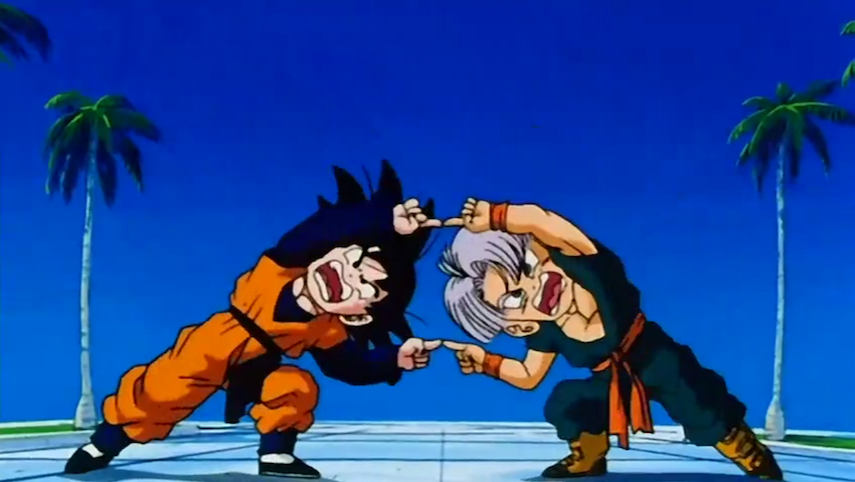
\includegraphics[scale=0.35]{resources/dbz-fusion.png}
			
			\tiny{\cite{dragonballz}}
		\end{figure}
	\end{frame}

	\begin{frame}
		\begin{figure}
			\centering
			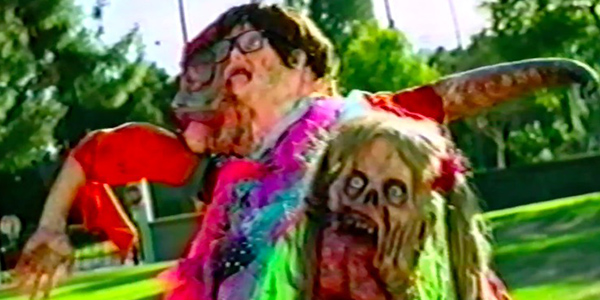
\includegraphics[scale=0.5]{resources/liquid-slam.jpg}
			
			\tiny{\cite{liquidslam}}
		\end{figure}
	\end{frame}

	\begin{frame}
		\begin{figure}[h]
			\centering
			\begin{tikzpicture}
			\tikzstyle{head} = []
			\tikzstyle{branch}=[draw, minimum size=25pt]
			\tikzstyle{commit} = [dash pattern=on 3pt off 3pt, draw, minimum size=25pt]
			\tikzset{edge/.style = {-,-> = latex}}
			
			\node[head](history)at (0,0) {...};
			\node[commit](commit3) at (3,0) {0de24};
			\node[commit](commit4) at (6,-1) {87fa1};
			\node[commit](commit5) at (6, 1) {76e0c};
			\draw[edge](commit3) to (history);
			\draw[edge](commit4) to (commit3);
			\draw[edge](commit5) to (commit3);
			
			\node[branch](master) at (6,2.5) {\texttt{master}};
			\draw[edge](master) to (commit5);
			
			\node[branch](testing) at (6,-2.5) {\texttt{testing}};
			\draw[edge](testing) to (commit4);
			
			\end{tikzpicture}
		\end{figure}
		Merge \texttt{testing} und \texttt{master}.
	\end{frame}

	\begin{frame}
		\frametitle{Three-Way-Merge}
		\begin{itemize}
			\item Merge \texttt{master} und \texttt{testing} mit Hilfe eines gemeinsamen vorhergehenden Knotens
			\item Erzeuge neuen Commit, der sowohl die beiden Commits als Elternknoten hat und verschiebe \texttt{master}.
			\item Lösche \texttt{testing}, da nicht weiter benötigt.
		\end{itemize}
	\end{frame}

	\begin{frame}
		\begin{figure}[h]
			\centering
			\begin{tikzpicture}
			\tikzstyle{head} = []
			\tikzstyle{branch}=[draw, minimum size=25pt]
			\tikzstyle{commit} = [dash pattern=on 3pt off 3pt, draw, minimum size=25pt]
			\tikzset{edge/.style = {-,-> = latex}}
			
			\node[head](history)at (0,0) {...};
			\node[commit](commit3) at (3,0) {0de24};
			\node[commit](commit4) at (6,-1) {87fa1};
			\node[commit](commit5) at (6, 1) {76e0c};
			\node[commit](commit6) at (9,0) {6ef23};
			\draw[edge](commit3) to (history);
			\draw[edge](commit4) to (commit3);
			\draw[edge](commit5) to (commit3);
			\draw[edge](commit6) to (commit4);
			\draw[edge](commit6) to (commit5);
			
			\node[branch](master) at (9,2.5) {\texttt{master}};
			\draw[edge](master) to (commit6);
			
			\end{tikzpicture}
		\end{figure}
	\end{frame}

	\begin{frame}
		\frametitle{Three-Way-Merge}
		\begin{itemize}
			\item Geht nicht immer ganz reibungslos $\rightarrow$ Merge-Konfilkte
			\item Git markiert die Stellen die in Konflikt stehen
			\item Manuelles lösen der Konflikte nötig
		\end{itemize}
	\end{frame}


	\begin{frame}
		\frametitle{Git Workflow}
		\begin{itemize}
			\item Änderungen an lokalem Branch vornehmen (\texttt{git add})
			\begin{itemize}
				\item Jeder Task sollte seinen eigenen Branch haben\\ (\texttt{git checkout -b BRANCH})
			\end{itemize}
			\item Lokale Snapshots erstellen (\texttt{git commit})
			\item Snapshots auf den Server laden (\texttt{git push})
			\item Merge mit \texttt{master}-Branch (\texttt{git merge BRANCH})
		\end{itemize}
	\end{frame}

	\begin{frame}
		\frametitle{Git Inside}
		\begin{itemize}
			\item Viele Dienste erweitern Git um eigene Funktion:
			\begin{itemize}
				\item Issue Tracker
				\item Code Dokumentation
				\item Merge-/Pull-Requests
			\end{itemize}
		\end{itemize}
	\end{frame}

	\begin{frame}
		\frametitle{Issue Tracker}
		\begin{itemize}
			\item Verwaltung von Feature-Requests und Bugs
			\item Diskussionsplattform
			\item Weise Issues Branches und Personen zu
		\end{itemize}
	\end{frame}

	\begin{frame}
		\frametitle{Merge-/Pull-Requests}
		\begin{itemize}
			\item Möglichkeit einen Merge zu beantragen
			\item Mehr-Augen-Prinzip: Merge muss angenommen werden
			\item Diskussion über Merge möglich
		\end{itemize}
	\end{frame}
	
	\begin{frame}
		\bibliographystyle{plain}
		\tiny\bibliography{literatur}
		\addcontentsline{toc}{section}{\bibname}
	\end{frame}
	
\end{document}
